\documentclass[11pt]{article}

% Page geometry
\usepackage[margin=0.4in]{geometry}

% Typography
\usepackage[T1]{fontenc}
\usepackage{microtype}
\usepackage{multicol}
% Math
\usepackage{amsmath,amssymb,amsthm}

% Figures and tables
\usepackage{graphicx}
\usepackage{booktabs}
% Figures and tables
\usepackage{subcaption}
\usepackage{float}

% Make section headings smaller
\usepackage{titlesec}
\titleformat{\section}{\normalsize\bfseries}{\thesection}{1em}{}
\titleformat{\subsection}{\small\bfseries}{\thesubsection}{1em}{}
\titleformat{\subsubsection}{\footnotesize\bfseries}{\thesubsubsection}{1em}{}

% Make title smaller
\makeatletter
\renewcommand{\maketitle}{%
    \begin{center}
        {\normalsize \@title}\par
        \vskip 0.5em
        {\small \@author}\par
        \vskip 0.5em
        {\small \@date}\par
    \end{center}
}
\makeatother

% Make figure and table captions smaller
% \usepackage[font=small,labelfont=bf]{caption}
% Algorithms
\usepackage{algorithm}
\usepackage{algorithmic}

% References and links
\usepackage[colorlinks=true,linkcolor=blue,citecolor=blue,urlcolor=blue]{hyperref}
\usepackage[numbers]{natbib}

% Theorem environments
\newtheorem{theorem}{Theorem}
\newtheorem{lemma}[theorem]{Lemma}
\newtheorem{proposition}[theorem]{Proposition}
\newtheorem{definition}{Definition}

% Useful shortcuts
\newcommand{\R}{\mathbb{R}}
\newcommand{\E}{\mathbb{E}}
\newcommand{\argmin}{\operatorname{argmin}}
\newcommand{\argmax}{\operatorname{argmax}}

\renewcommand{\abstractname}{Summary}

\usepackage{xcolor}

% Make blockquotes italic and gray with a line at the end
\let\oldquote\quote
\let\endoldquote\endquote
\renewenvironment{quote}{\oldquote\itshape\color{gray}}{\par\noindent\rule{\linewidth}{0.4pt}\endoldquote}


\title{Mo Memory Mo Problems: Vision Foundation Models for Digit Classification}
\author{Arjun Sharma\\
\texttt{asharma3@caltech.edu}}
\date{}

\begin{document}

\maketitle

\textit{My code for this project is visible at \url{https://github.com/ArjunS07/cs-148/project4}.}


\section{CLIP zero-shot run}

I achieved 21.5\% accuracy with a zero-shot CLIP approach.

\textbf{CLIP}. The original training setup for CLIP \cite{radford2021learning} adopted a contrastive learning framework. Given a batch of $N$ image-caption pairs sourced from the internet, CLIP's text and image encoders are trained together to embed images and captions in the same space such that the $N$ cosine similarities of matching images and captions is maximized and the $N^2 - N$ cosine similarities of non-matching images and captions is minimized. This is formalized as a symmetric cross-entropy loss acros each row and column. A trained CLIP model is therefore capable, in theory, of embedding images and text in a semantically meaningful embedding space where correspondences can be straightforwardly calculated.

The specific CLIP instance used in my experiments was \texttt{clip-ViT-B-32} from Hugging Face, which has a total of 151,277,313 total parameters: 87,456,00 parametrs for its vision encoder, 63,165,952 parameters for its text encoder, and a remaining 655,361 parameters for its projection layers.

\textbf{Setup}. I used a prompt ensembling approach. Text embeddings of each of the below prompt templates was extracted for each digit. An `average text embedding' was extracted for each digit through a simple mean of all of its prompts. Then, following the template, classification of an image was done by returning the digit whose prompt had the highest cosine similarity with the image's CLIP embedding.

The prompts used, for each digit, were:
\begin{verbatim}
    "a photo of the number: "{}". ", "a handwritten digit {}", "the number {} written on paper", 
    "an image of the digit {}", "a photo of {} written by hand", "a close-up of the number {}",
     "the digit {} in a natural setting", "a difficult photo of the number {}",
     "a noisy image of the digit {}"
\end{verbatim}


\textbf{Results}. Analysis is presented in the captions of \autoref{fig:clip-zs-confusion-mat} and \autoref{fig:clip-worst-examples}.

\begin{figure}[H]
    \centering
    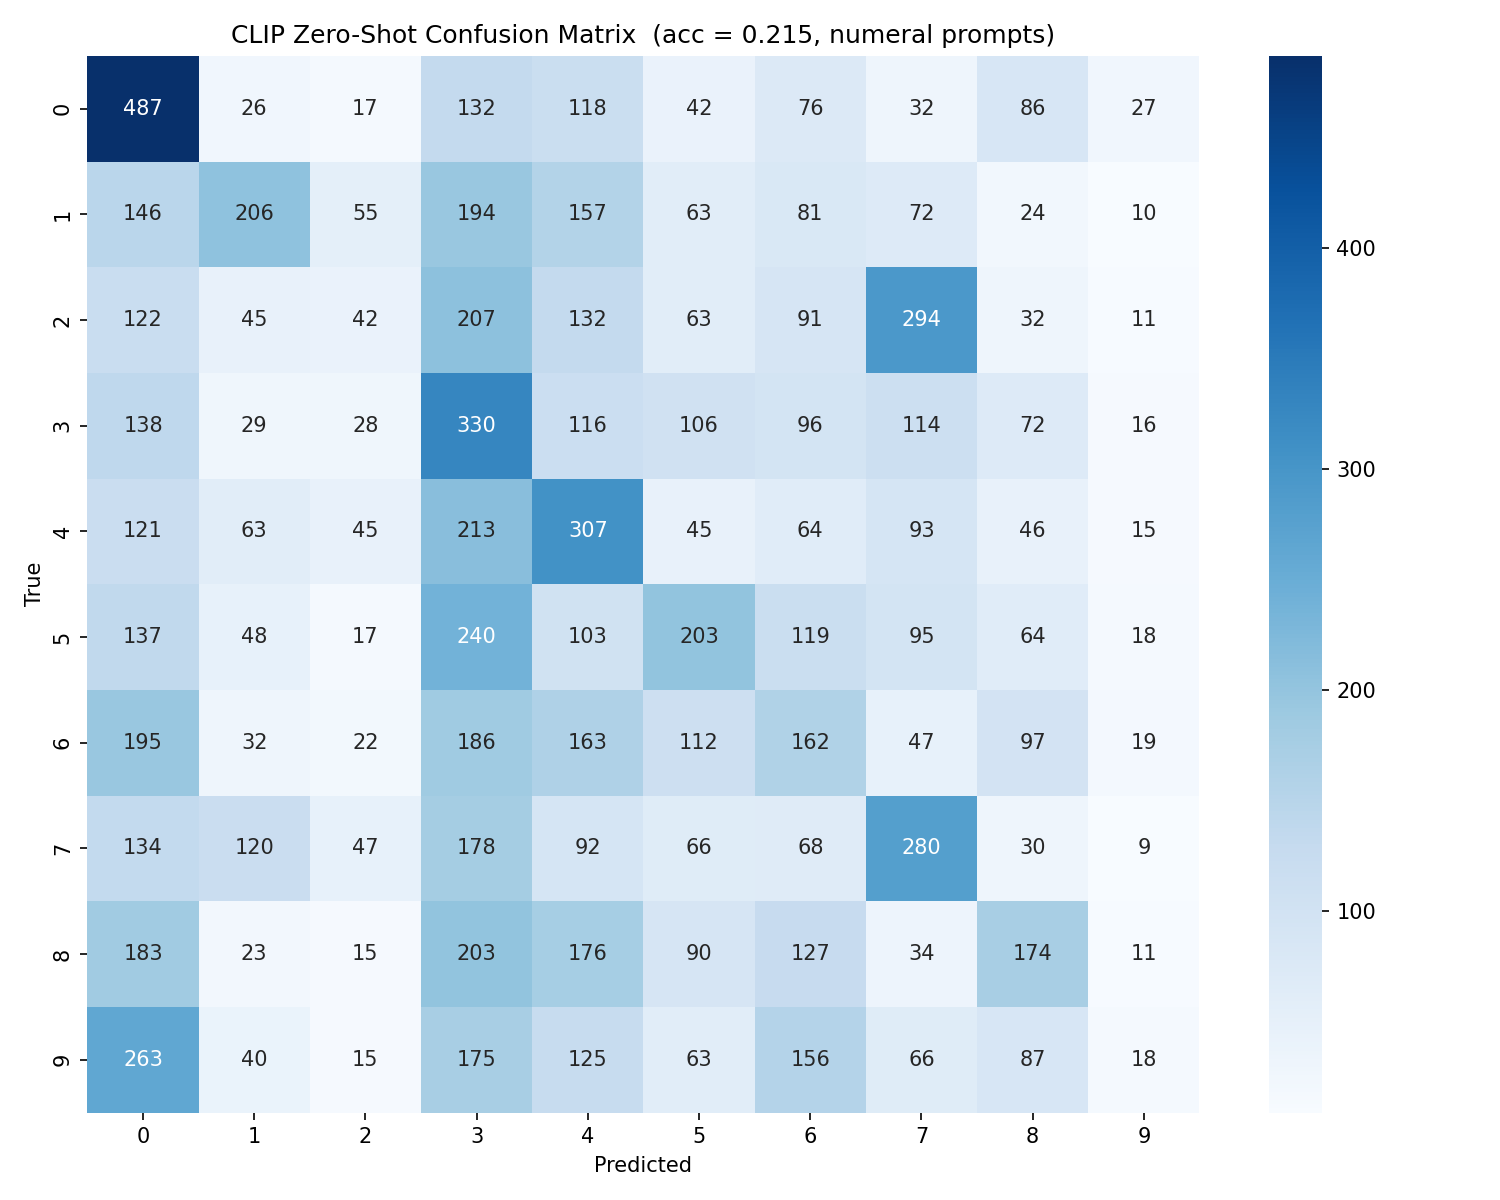
\includegraphics[width=0.6\textwidth]{figures/clip_zs/confusion_matrix.png}
    \caption{Confusion matrix for zero-shot CLIP classification. CLIP has a strong bias to predicting the labels 0 and 3 in this dataset and against predicting 2 and 9. It is best for globally geometriocally distinct shapes like 4 and 5. Overall performance is poor.}
    \label{fig:clip-zs-confusion-mat}
\end{figure}

\begin{figure}[H]
    \centering
    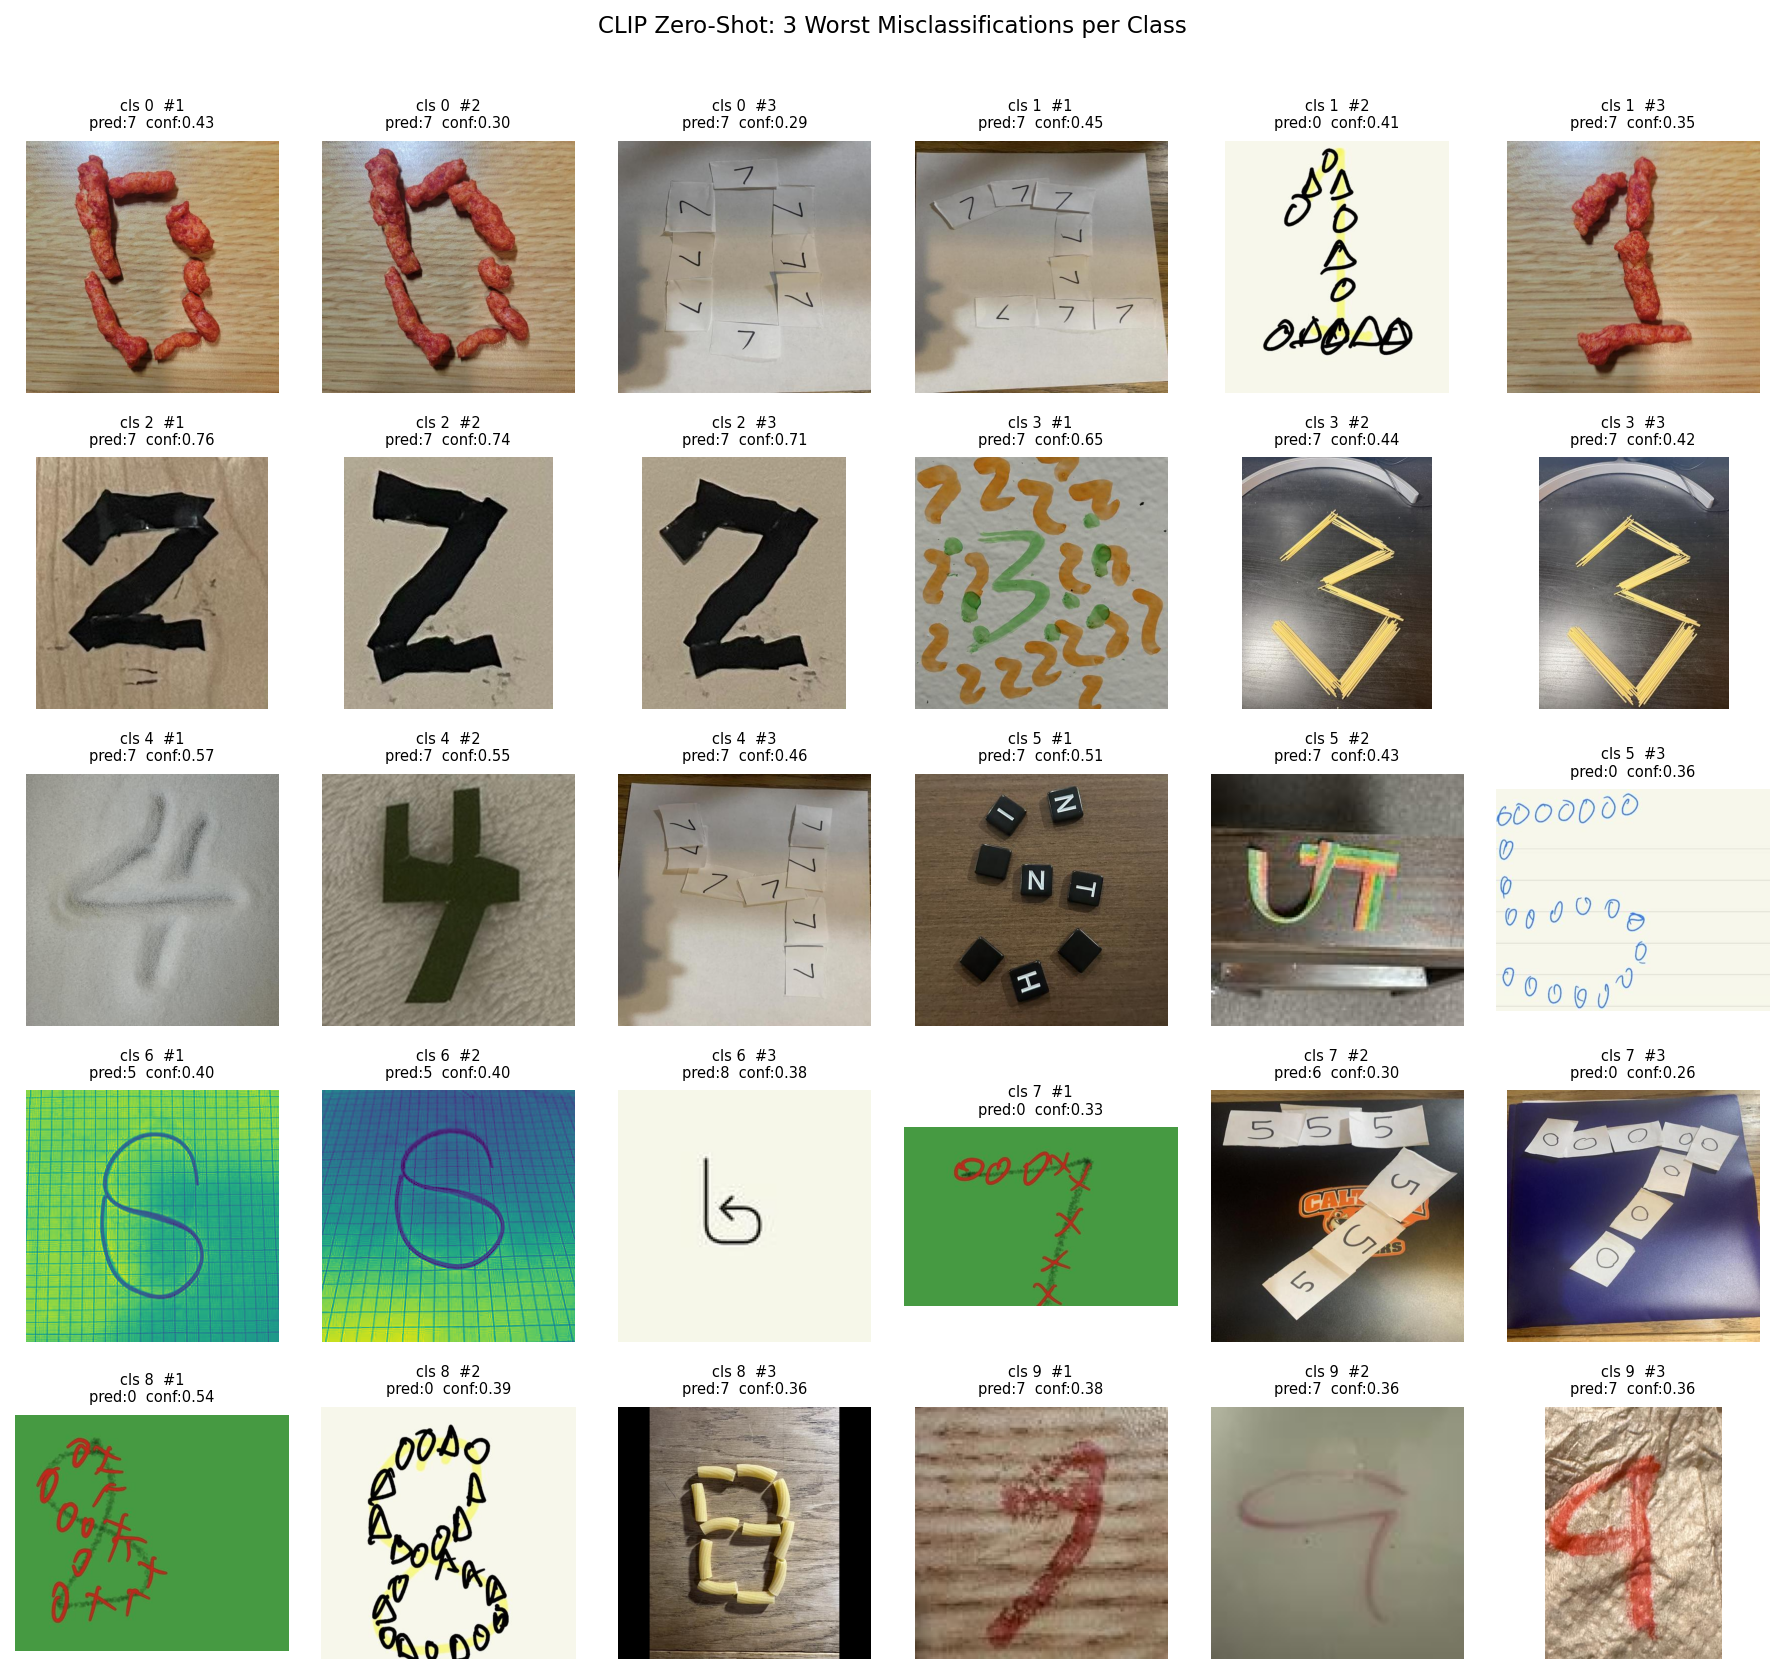
\includegraphics[width=0.6\textwidth]{figures/clip_zs/worst_per_class.png}
    \caption{3 worst CLIP predictions per class, i.e., incorrect predictions with the highest cosine similarity between the predicted label and image. A few datasets in particular dominate. Note the bias towards predicting 7, likely due to local geometric features like sharp bends being best correlated with 7s in the training distribution. Also note how CLIP is fooled by the dataset which arranges local digits like 5 or 0 into a global structure. It is similarly confused by the geometry of the three six examples, mistaking the sparsity in the first two for a 5. }
    \label{fig:clip-worst-examples}
\end{figure}

I additionally tested nearly-identical prompts using words for numbers instead of literal digits (eg. `one' instead of 1), and achieved only 16.3\% accuracy using words, which aligns with the official CLIP recommendations for MNIST datasets and makes sense since CLIP was trained on uncurated internet captions which are more likely digits. 

\section{Downstream Models}

\begin{figure}[H]
    \centering
    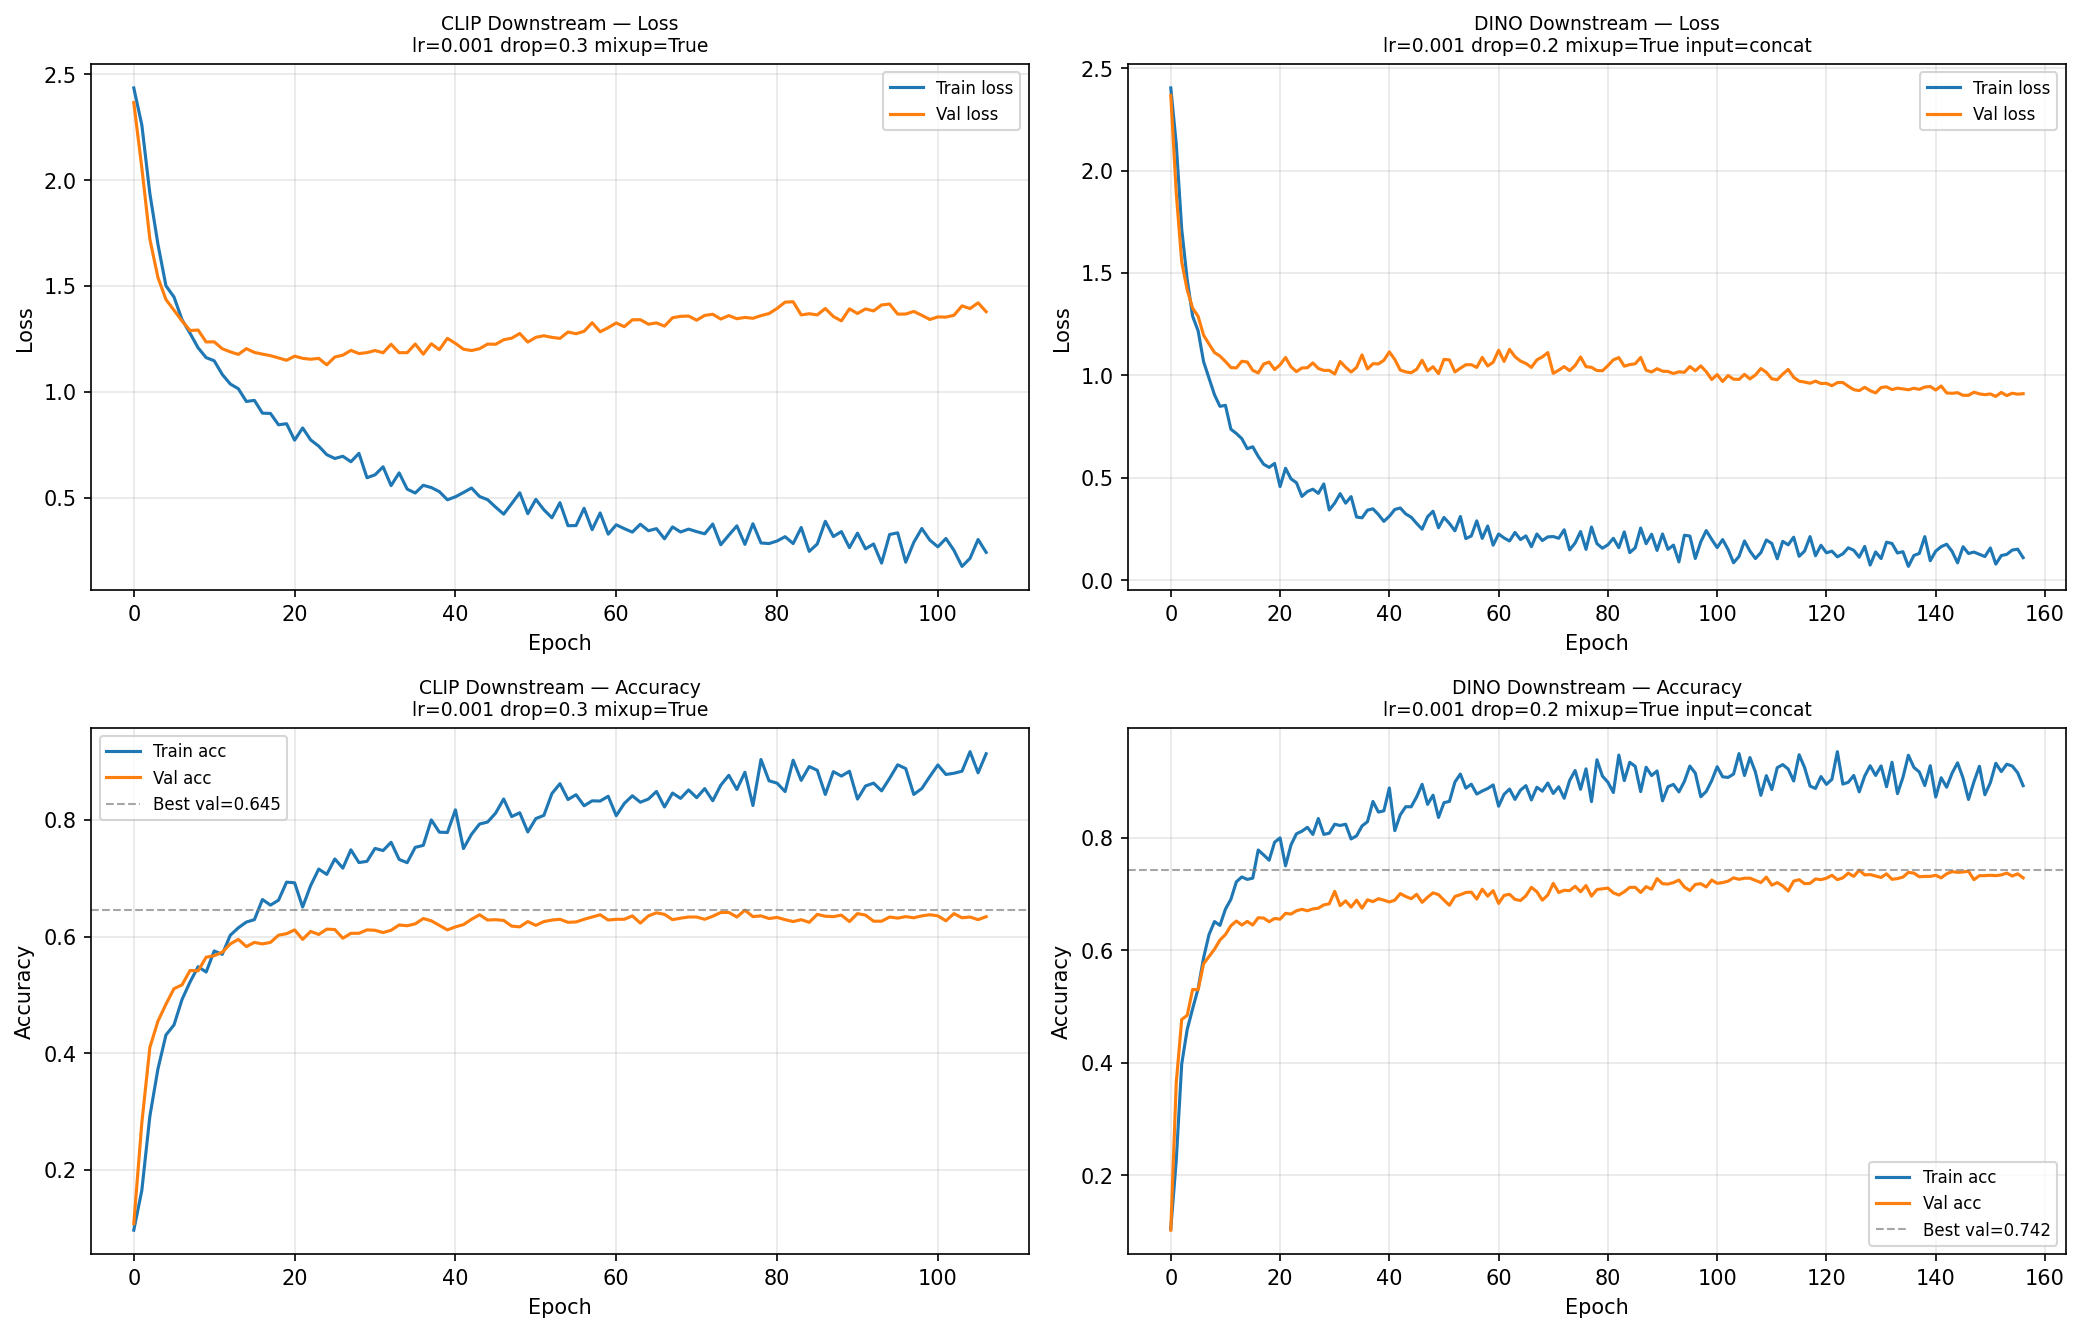
\includegraphics[width=\textwidth]{figures/downstream/training_curves.png}
    \caption{Training curves across all downstream models tested. We notice a significant degree of overfitting. }
    \label{fig:loss-curves-downstream}
\end{figure}

\subsection{CLIP Downstream Model}

\textbf{Model training setup}. I froze the parameters of ther CLIP foundation model and trained a simple neural network which took in the CLIP embedding of an image and produced 10 outputs, specifically, it was a 3-layer MLP with the form  
Linear(512, 256) $\to$ BatchNorm1d(256) $\to$ ReLU $\to$ Dropout $\to$ Linear(256, 128) $\to$ BatchNorm1d(128) $\to$ ReLU $\to$ Dropout $\to$ Linear(128, 10). I used cross-entropy loss since that is the standard loss for classification and has the effect of automatically applying a softmax-like effect. I used the AdamW optimizer with weight decay $10^{-4}$.

\textbf{Learning rate and batch size}. During training, I used a cosine warmup learning rate schedule with 5 warmup epochs and a minimum learning rate of $10^{-3}$. 

I swept learning rates over $10^{-3}, 3 \times 10^{-4}, 10^{-4}$ and found that the highest - $10^{-3}$ worked best. However, accuracy was not significantly impacted by these choices. It was 0.632, 0.638, and 0.641 respectively for each of these choices. 

Taking into account previous experience running these models on my laptop, and following established heuristics, I used a batch size of 64 during training. 

\textbf{Training and epochs}. I trained for a maximum of 200 epochs with early stopping set to patience 30 epochs. The best CLIP model converged by epoch 106, so 200 was a generous upper bound set during experiments. Loss and accuracy curves are presented in \autoref{fig:loss-curves-downstream}. We achieve a maximum validation accuracy of 64.5\%, whose checkpoint is restored for future experiments. 

\textbf{Validation strategy}. Continuing my previous setupo, I perform a stratified 85:15 split by label, thus ensuring each digit class has equal representation in val. No validation images were ever used for embedding extraction choices or architecture design.

\textbf{Overall choices}. This approach of applying an MLP head to the embedding extraction layer makes sense under the premise that CLIP is already doing the work of extracting a useful representation of the image, the way a CNN or ViT in the previous projects is trained from scratch to do, so we essentially just need a smalll `decoder' to convert this representation into a digit prediction. I chose not to implement augmentations because I tried aggressive augmentations, borrowing from my previous two projects, beforehand, but they hurt classification accuracy, which makes sense since they likely significantly degraded the CLIP representation quality passed to the MLP and were too difficult to recover from after the highly complex transformation applied by CLIP. I tested both BatchNorm and LayerNorm and found BatchNorm to perform much better. 

\textbf{Differences with respect to previous projects}. In this paradigm, there is no end-to-end training as there was for the CNN and ViT where models were trained from scratch. Here, we freeze the encoder and use those features for a small downstream model. Experimental details such as augmentations change as a result (they were crucial for previous projects and not helpful here), as does the sensitivity to factors such as learning rate. Training time here is minimal compared to the CNN or ViT. The overall parameter count here is an order of magnitude if we count the CLIP model size relative to the CNN or ViT, which were on the order of 5-10M. 

\subsection{DINO Downstream Model}

\textbf{DINO Model}. The DINO model used here, \texttt{dino-v2-base} has 86,580,480 parameters. The original training setup \cite{caron2021emerging} was a self-supervised one: a student model, with access to local views of an image, was trained to mimic the outputs of a teacher model, which had access to global views of the image; the teacher's weights were updated using an exponential moving average of the gradients received by the student. 

\textbf{Model setup}. I tried two approaches: operating on the CLS token directly, and operating on (CLS + a mean of the patch embeddings produced by the DINO). The first model had 346,890 parameters and the second had 855,178 parameters, which are tiny compared to the size of DINO itself. 

Other design choices were the same, and the same learning rate was found to be the best for DiNO as for the CLIP model.

\textbf{Validation performance}. DINO-downstream outperforms CLIP-downstream. The (CLS + patch mean) approach achieved a validation accuracy of 74.2\% on the same dataset (the CLS-only approach also outperformed CLIP, but to a lesser degree, achieving 72.0\% accuracy). 

Training curves are provided side-by-side with the CLIP model in \autoref{fig:loss-curves-downstream}. Performance saturates around the same time and overfitting degradation does not occur to the same extent in the DINO model.

\textbf{Qualitative comparison}. Empirical analysis shows that DINO outperforms CLIP for every class. Examples of differences in their output are shown in \autoref{fig:examples-dino-corr-clip-wrong} and \autoref{fig:examples-dino-wrong-clip-right}.

\begin{figure}[H]
    \centering
    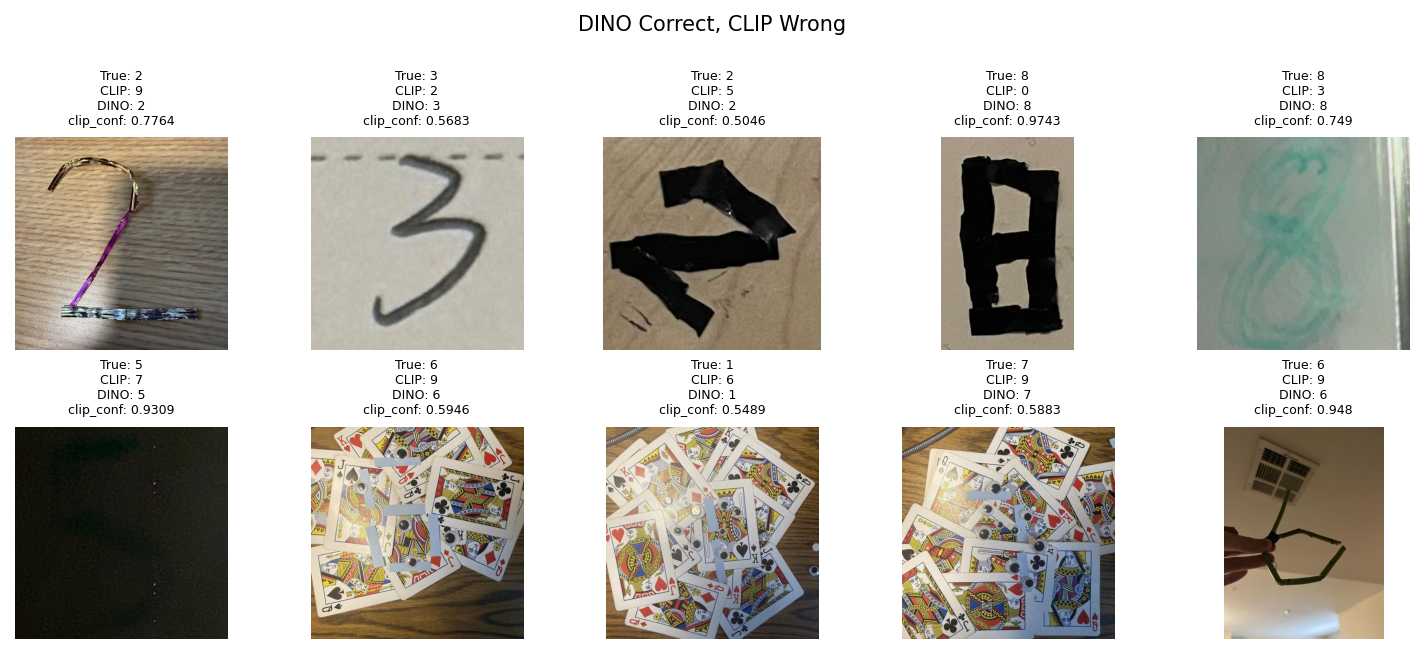
\includegraphics[width=0.9\textwidth]{figures/downstream/dino_right_clip_wrong.png}
    \caption{Examples where DINO-downstream was correct and CLIP-downstream was wrong}
    \label{fig:examples-dino-corr-clip-wrong}
\end{figure}

\begin{figure}[H]
    \centering
    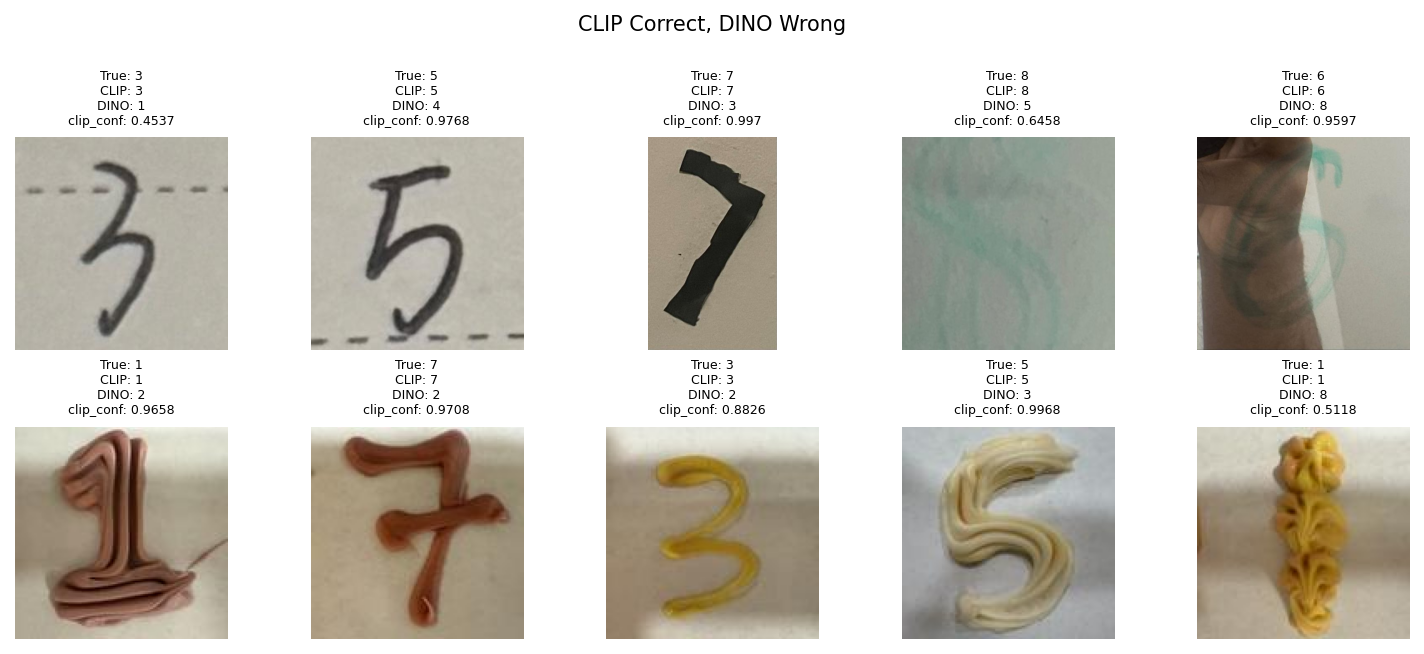
\includegraphics[width=0.9\textwidth]{figures/downstream/clip_right_dino_wrong.png}
    \caption{Examples where CLIP-downstream was correct and DINO-downstream was wrong. Many of the examples here are less globally noisy than the average sample in the distribution.}
    \label{fig:examples-dino-wrong-clip-right}
\end{figure}

DINO seems to perform better in attending to salient local structure in a noisy environment, most prominently seen in the card examples. However, looking to, for example, the last two examples in each row in \autoref{fig:examples-dino-wrong-clip-right}, we see that DINO gets distracted by local geometry such as curves.

We can link these to the original training objectives. CLIP is trained via image-text contrastive learning only so it is trained to emphasize global semantic structure corresponding to the captions, such that it works well on clean digits when the overall shape aligns well with semantic concepts but fails with structurally unusual cases. DINO, in contrast, is trained with multi-view augmentations such that it is sensitive to local geometric features and relatively invariant to distortions, such that it succeeds on cluttered digits by focusing on local digit structure. However, this structural bias likely causes it to fail when particular parts of the image produce features corresponding to other digits. 

\section{Autorgressive Qwen VLM}

My code for this portion is available at \url{https://colab.research.google.com/drive/1_C9SqGFbcU8svi_EDTGZTWOh_S3XeV5X?usp=sharing}

\textbf{Qwen model}.

I used \texttt{Qwen/Qwen2.5-VL-3B-Instruct}, which has 4.1 billion total parameters including its vision encoder, vision language adapater, and LLM decoder. 

It uses byte pair encoding and splits digits into special characters, such that each digit in a number is its own token. It uses special tokens for the beginning of a turn (\texttt{<|im\_start|>}) and the end of a turn (\texttt{<|im\_end|>}), using special tokens to mark the \texttt{user}, \texttt{assistant}, and \texttt{system}. 

A ViT is used for image preprocessing, using an architecture which scales the number of tokens with respect to image suize. This prevents the need for fixed size cropping. 

The training setup takes three stages: first, a vision encoder is trained on text-image pairs to establish a multimodal representation space; then, model parameters are trained on a broad dataset with images, OCR, visual question answering, and diverse document formats; finally, the vision encoder weights are frozen and the lanaguage model is curated on an instruction following dataset. Finally, supervised fine tuning on chat responses is employed followed by reinforcement learning. 

\textbf{Results}. I achieve 35.3\% accuracy on images with the following prompt:

\begin{quote}
    Look carefully at this photograph. Hidden somewhere in the image is a single handwritten digit from 0 to 9. What is that digit? Reply with only the digit.
\end{quote}

Results were extremely sensitive to the prompt. A previous prompt resulted in it almost always outputting 0 or 9. Another prompt caused it to output too many tokens (restricting max tokens to 2 and being more aggressive in instructions helped). 

The VLM overall performs poorly. We visualize results below.

\begin{figure}[H]
    \centering
    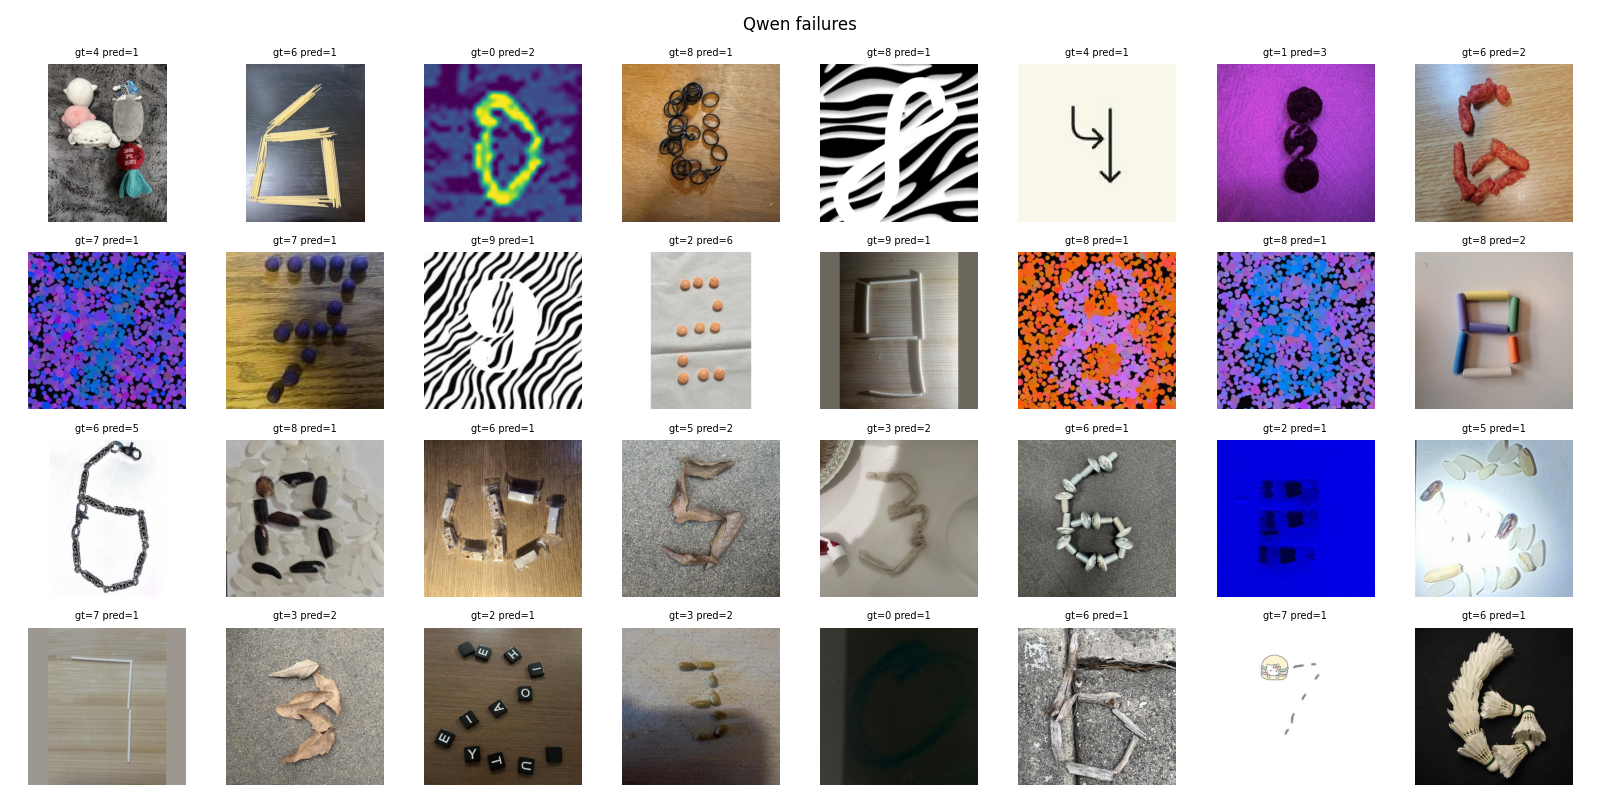
\includegraphics[width=0.75\textwidth]{figures/figs-qwen/qwen_fail.png}
    \caption{Images on which the Qwen VLM failed. Broadly, these are just the long tail of adversarial examples in this dataset. It fails due to distortions, color changes, adversarial settings such as too much noise, etc. }
\end{figure}

Interestingly, it is particularly biased to certain labels. \begin{figure}[H]
    \centering
    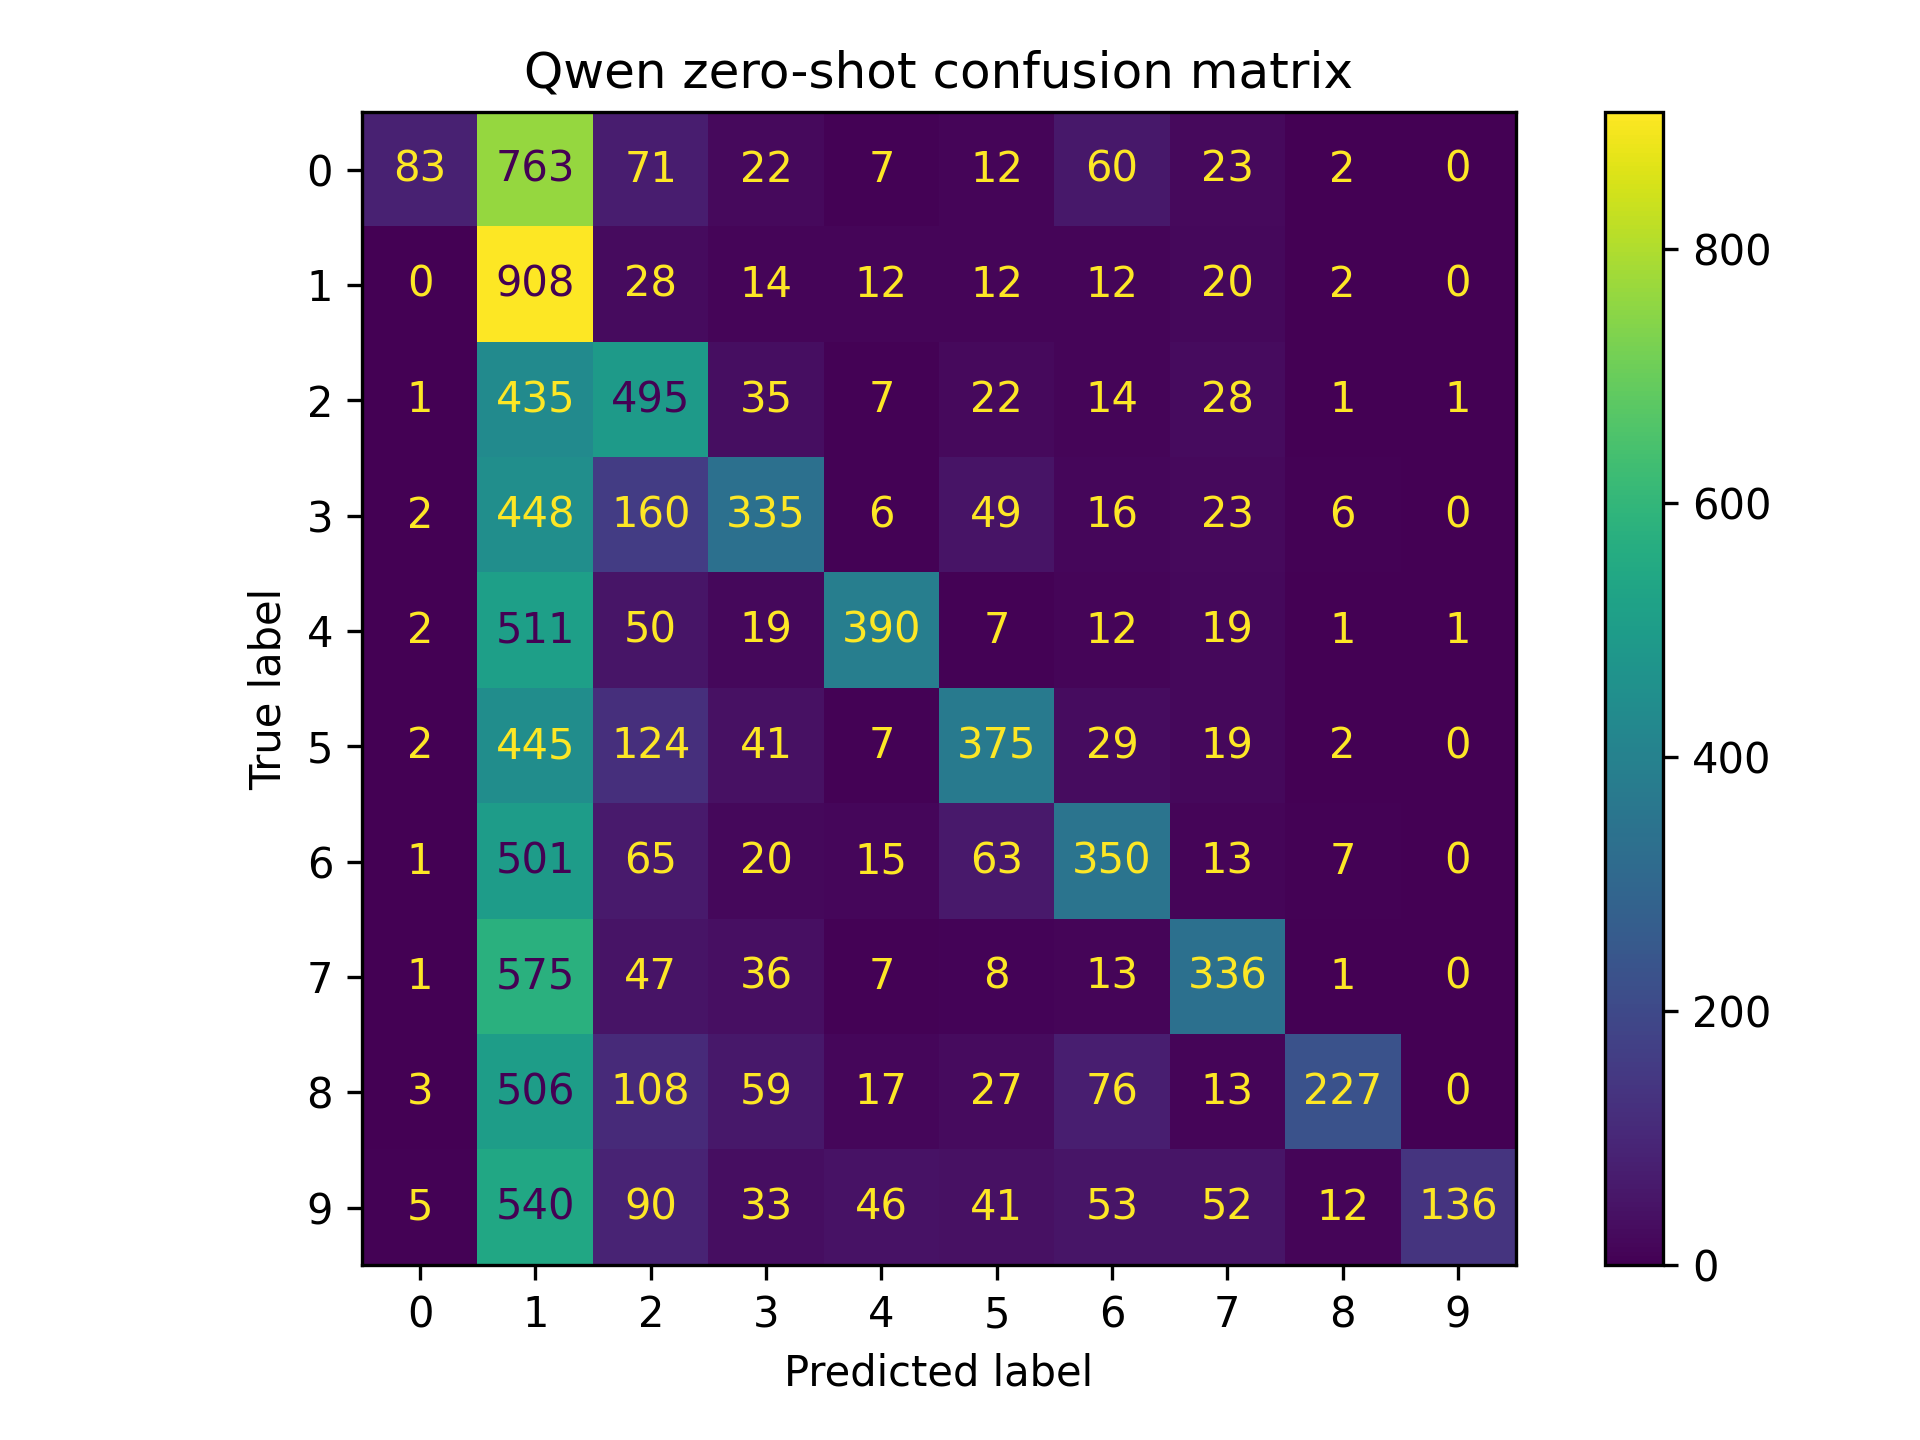
\includegraphics[width=0.4\textwidth]{figures/figs-qwen/qwen_confusion_matrix.png}
    \caption{The VLM is biased towards consistently predicting 1. This is likely because it has not been trained as a classifier and 1 probably appears frequently as the next token in its corpus. When data is noisy, it likely just defers to predicting 1.}
\end{figure}


\section{Overview and conclusion}

By far, my ResNet CNN performed the best, achieving 96.00\% validation accuracy with optimal hyperparameters. My DINO-downstream achieved 74.2\%, ViT achieved 72.9\% accuracy, CLIP-downstream achieved 64.5\%, zero-shot Qwen VLM achieved CLIP achieved 35.31\%, and zero-shot CLIP achieved 21.5\%. 

Clearly, task-specific training works best: there is a clear separation between trained models and zero-shot foundation models. The CNN's advantage emerges from it being fundamentally well adapated to the relatively sparse data regime due to it imposing strong inductive biases and learning a high-quality feature space under distortion, which the ViT struggles to learn. The general CLIP and DINO models do not have feature spaces well adapated to this regime: the quality of the MLP is limited by the encoders never being trained to learn robust representations in the manner necessary for this dataset. The Qwen model outperforms CLIP likely due to better instruction-following and image grounding during pretraining, but both models are underfit for this adversarial regime and must use their general emebedding space which likely is far shifted from the distribution of these images. 

\bibliographystyle{plainnat}
\bibliography{refs}


\appendix
\section{AI Usage}

Prompts are provided below. I set up a session with Claude web for lit review and planning, and manually wrote a plan.md document which I gave to Claude code, which then implemented files necessary (many were slight edits to files I gave it from previous projects, eg. the dataloader and visualization scripts).

\begin{enumerate}
    \item I've attached the guideliens for a project and the skeleton of a starter notebook provided by the class for this project. This is the third phase of this project - the first phase was building a CNN for this same dataset, and the second was on using a ViT.  I'm attaching my report for the CNN for context (I got 95% accuracy with ResNet).

Note that the data here is very adversarial. It's not at all like standard MNIST. 

Now, I haev to use foundation models - CLIP and DINO - for classification. The example notebook tries the following for CLIP - zero shot first, and then a downstream classification head.I need to do both of these with high performance, and then do a DINO downstream model as well.


Let's start by doing literature review. Analyze what problems we're likely to face here considering the kind of data. Do literature review on how to get good zero-shot CLIP performance, and then do extensive literature review on how to do downstream classification with CLIP and DINO. Find general techniques and also find techiques suited to each of these models in particular.

Note that we're relatively GPU constrained and have about $30$ in colab GPU credits. The goal is to try to survey techniques which do not add an unreasonable amount of  computational overhead.

\item 1. I tried distillation from my ResNet to my ViT earlier, and while the raw Resnet got 95\% performance and a vit got 75\%, the distilled ViT got stuck around 55\%. Analyze whether distillation from resnet would be useful here for the downstream classifiers.
2. Do a similar literature review for the extra credit section for Qwen. It seems like the main issue will be prompt engineering.

\item If I'm on an M5 mac, how computationally expensive will training or inference be here?


\item Analyze the extent to which synthetic data, as described in project 2, is likely to work here. How helpful would data scaling be? We found a 3\% accuracy improvement with an injection of synthetic data equal in size t1o 60\% of the original dataset with the CNN

\item I have decent proof that the synthetic images for the resnet CNN - if you look at the features of the final layer, the synthetic data, augmented data, and original data cluster well together.

\item Examine the augmentations I used previously for the CNN:

\textit{Python code ommitted for latex document}

Which one of these makes sense? Should I use separate ones for the CLIP and DINO models?

\item Review this plan for a coding agent

The plan was:
\begin{verbatim}
    
This is guidance for a deep learning class project. The goal is to build a multi(10)-class classifier using foundation models for extremely adversarial digit data, using a dataset of 10,000 examples.

The exact guidelines for this project are in project_instructions.md. A previous project, which is in ../project2/, consisted of building a CNN for this same dataset, which achieved 95% accuracy. The report describing that attempt is in this directory in report2_cnn_mnistw_tex_source.txt.

There are 3 main tasks which need to be accomplished for this project:
1. Zero-shot CLIP classifier
2. CLIP downstream classifier eg. with an MLP classification head that operates on CLIP latents
3. SAM downstream classifier eg. similarly using an MLP head

The starter notebook for this project is in CS148a_proj4_FM_starter.ipynb. I have run the dataset generation code in it already, whose output is loading in data/ right now. `data.py` contains the dataloader used for project 2, where I used synthetic data. At minimum, we'd use the Provided Digit Dataset loader from project 2. 

The starter notebook contains this configuration for CLIP and DINO, which we must use
```
from transformers import CLIPProcessor, CLIPModel
import torch

# Loading CLIP
print("Loading CLIP B32...")
clip_model = CLIPModel.from_pretrained("openai/clip-vit-base-patch32")
clip_processor = CLIPProcessor.from_pretrained("openai/clip-vit-base-patch32")
print("CLIP B32 loaded successfully.")

#make sure you freeze the clip model

clip_model.eval()
for param in clip_model.parameters():
    param.requires_grad = False


from transformers import AutoImageProcessor, AutoModel

# Loading DINOv2
print("Loading DINOv2 Base...")
dino_model = AutoModel.from_pretrained("facebook/dinov2-base")
dino_processor = AutoImageProcessor.from_pretrained("facebook/dinov2-base")
print("DINOv2 Base loaded successfully.")

# Freeze the DINO model
dino_model.eval()
for param in dino_model.parameters():
    param.requires_grad = False
```

We will write all our code in src/, store experiment results in checkpoints/, log experiments in logs/. All experiments will be run locally on this device, which is an M5 Macbook Pro with MPS.

The plan for this project is as follows:
1. Cache CLIP text embeddings of, for each digit, the captions
```
"a photo of the number: \"{}\"."
"a handwritten digit {}"
"the number {} written on paper"
"an image of the digit {}"
"a photo of {} written by hand"
"a close-up of the number {}"
"the digit {} in a natural setting"
"a difficult photo of of the number {}"
"a noisy image of the digit {}"
```
Average the L2-normalized text embeddings across all templates for each class.

2. Apply the augmentations in about this pseudocode for this dataset, applying K = 4 augmentations per image randomly.
    ```
    from PIL import Image

    def get_augmentation_for_fm():
        """Apply BEFORE the model's processor. Works on PIL images."""
        return transforms.Compose([
            transforms.RandomResizedCrop(224, scale=(0.7, 1.0), ratio=(0.75, 1.33)),
            transforms.RandomRotation(10),
            transforms.ColorJitter(brightness=0.2, contrast=0.2, saturation=0.2, hue=0.05),
            transforms.GaussianBlur(kernel_size=3, sigma=(0.1, 1.0)),
        ])

    # Then for CLIP:
    aug_image = get_augmentation_for_fm()(pil_image)
    inputs = clip_processor(images=aug_image, return_tensors="pt")
    embedding = clip_model.get_image_features(**inputs)

    # For DINO:
    aug_image = get_augmentation_for_fm()(pil_image)
    inputs = dino_processor(images=aug_image, return_tensors="pt")
    outputs = dino_model(**inputs)
    embedding = outputs.last_hidden_state[:, 0, :]
    ```
3. Cache CLIP and DINO embeddings for the augmented images. We'll use these for all future experiments to speed things up.
4. Set up the pipeline for the zero shot CLIP classifier. Use the averaged text embedding.
5. Set up the downstream CLIP and DINO classifiers.
For CLIP:
```
512 → 256 → BatchNorm → ReLU → Dropout(0.3) → 128 → BatchNorm → ReLU → Dropout(0.3) → 10
```
for DINO:
```
768 → 384 → BatchNorm → ReLU → Dropout(0.3) → 128 → BatchNorm → ReLU → Dropout(0.3) → 10
```
do the following:
* Batch normalization before each activation
* Dropout (0.2)
* Weight decay in AdamW optimizer, learning rate 3e-4 with warmup and decay. 

For the DINO downstream classifier, 
> For classification tasks using DINOv2, constructing input representations by concatenating the class token with the mean of the patch tokens ResearchGate can improve performance. Instead of just using outputs.last_hidden_state[:, 0, :] (CLS token, 768-dim), try also averaging patch tokens and concatenating: this gives you a 1536-dim input. This captures both global (CLS) and local (patch average) information.

Look to `project2_train.py.txt` in this directory for an idea of how to structure the training setup

Use label smoothing in the exact same way as `project2_train.py.txt`
\end{verbatim}

\end{enumerate}

For Claude code:
\begin{enumerate}
    \item Review guidance/agent\_guidance.md and ask clarifying questions
    \item 1. ProvidedDigitDataset. 2. Use integer indices 3. create embeddings 4. Write all scripts and write a command in a docstring at the top of each file. 5. Stop after writing. 6. ignore main.py 7. ignore the summary table command
    \item To improve zoer-shot performance, evaluate whether it would be better to extract the embeddings of the word corresponding to the digit and not the digit itself. Like one not 1   
    \item  Okay it's overfitting significantly wiht both config 0 and 1 - look at all\_Curves in checkpoints/clip\_downstream. Don't make any changes for now, but suggest future modifications to reduce overfitting risk. Mixup and a higher dropout value don't reduce       
  overfitting.       
\item         In addition to all your suggestions, let's also make the augmentations more aggressive.                                                                                   \item     nope remember dino used to be 76. let's roll back all the changes we made since we first observed overfitting                     

\end{enumerate}


\end{document}